\documentclass{article}
\usepackage{amsmath}
\usepackage{tikz}
\usepackage[margin=1in]{geometry}
\usepackage{amssymb}
\usepackage{caption}



\usetikzlibrary{calc, arrows.meta, angles, quotes, decorations.markings}


\setlength{\parskip}{4pt}
\title{Cars 4 -- Lightnight McQuation}
\author{Rhitt C}
\date{Feb 2026}


\begin{document}
\maketitle

\section*{Abstract}
Lightning McQueen, old and rusty, decides to officially retire from the racing scene, leaving Cruz to carry on his legacy.

In search of a new career, he thinks back to all the crazy stunts he'd pulled over the years and realises he has no idea how they were even possible physically.
So he has a crazy idea: why not become a physicist and research stunt mechanics?

Who knows, maybe a strong understanding will lay the foundations for a future NASCAR training business $\dots$

Note to self: learn simulink and experiment further with simulations

\section{The Basics of Friction -- Walking}

\section{First Paradigm -- Skidding and Drifting}

\section{Second Paradigm -- Banked Tracks}

\subsection{Deriving a general formula for Friction and Normal forces}

For ease of calculation, we deal with both friction down the slope (\textbf{Case 1}) and up the slope (\textbf{Case 2}) at once using ($\pm$) and ($\mp$).

Throughout the calculations, the sign on top (i.e. ($+$) in ($\pm$) and ($-$) in ($\mp$)) is for \textbf{Case 1} and the sign on the bottom is for \textbf{Case 2}.

\begin{figure}[h]
\centering
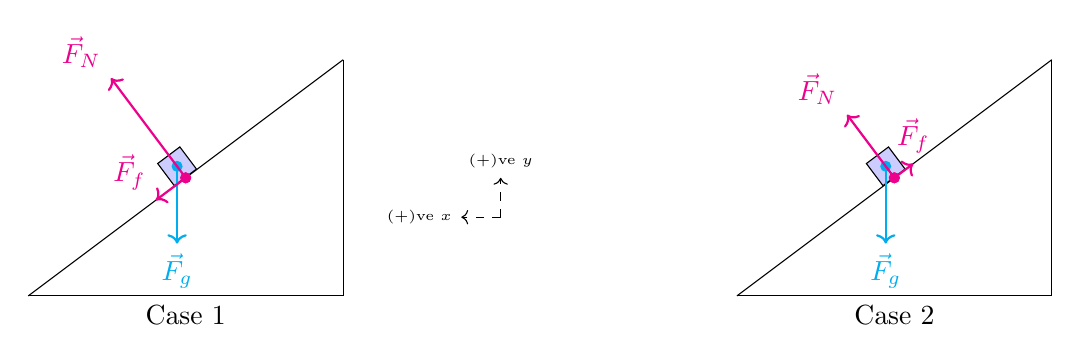
\begin{tikzpicture}
    \pgfmathsetmacro{\radius}{2}
    \pgfmathsetmacro{\g}{9.81}
    \pgfmathsetmacro{\mass}{0.1}
    \pgfmathsetmacro{\incline}{atan(3/4)}
    \pgfmathsetmacro{\fric}{0.3}
    \pgfmathsetmacro{\speed}{sqrt(\radius * \g * (  (tan(\incline)+\fric)/(1-\fric*tan(\incline))  ))}

    \draw (0, 0) -- (4, 0) node[midway, below] {Case 1} -- (4, 3);
    \draw (4, 3) -- (0, 0) node[midway, above, sloped, draw, fill=blue!20, minimum size=10pt] (c) {};


    \draw[dashed, ->] (6, 1) -- (6, 1.5) node[above, font=\tiny] {$(+)\text{ve }y$};
    \draw[dashed, ->] (6, 1) -- (5.5, 1) node[left, font=\tiny] {$(+)\text{ve }x$};


    
    \pgfmathsetmacro{\Fg}{\mass * \g}
    \fill[cyan] (c.center) circle (2pt);
    \draw[cyan, thick, ->] (c.center) -- ++(0, -\Fg)
        node[below] {$\vec{F}_g$};

    \pgfmathsetmacro{\FN}{\mass * ((\speed^2 * sin(\incline) / \radius) + (\g * cos(\incline)))}
    \fill[magenta] (c.south) circle (2pt);
    \draw[magenta, thick, ->] 
        (c.south) -- ++({\FN*cos(\incline+90)},{\FN*sin(\incline+90)})
        node[above left] {$\vec F_N$};

    \pgfmathsetmacro{\Ff}{\mass * ((\speed^2 * cos(\incline) / \radius) - (\g * sin(\incline)))}
    \fill[magenta] (c.south) circle (2pt);
    \draw[magenta, thick, ->] 
        (c.south) -- ++({\Ff*cos(\incline+180)},{\Ff*sin(\incline+180)})
        node[above left] {$\vec F_f$};




    \pgfmathsetmacro{\speedd}{sqrt(\radius * \g * (  (tan(\incline)-\fric)/(1+\fric*tan(\incline))  ))}


    \draw (9, 0) -- (13, 0) node[below, midway] {Case 2} -- (13, 3);
    \draw (13, 3) -- (9, 0) node[midway, above, sloped, draw, fill=blue!20, minimum size=10pt] (s) {};


    \fill[cyan] (s.center) circle (2pt);
    \draw[cyan, thick, ->] (s.center) -- ++(0, -\Fg)
        node[below] {$\vec{F}_g$};

    \pgfmathsetmacro{\FNN}{\mass * ((\speedd^2 * sin(\incline) / \radius) + (\g * cos(\incline)))}
    \fill[magenta] (s.south) circle (2pt);
    \draw[magenta, thick, ->] 
        (s.south) -- ++({\FNN*cos(\incline+90)},{\FNN*sin(\incline+90)})
        node[above left] {$\vec F_{N}$};

    \pgfmathsetmacro{\Fff}{\mass * ((\speedd^2 * cos(\incline) / \radius) - (\g * sin(\incline)))}
    \fill[magenta] (s.south) circle (2pt);
    \draw[magenta, thick, ->] 
        (s.south) -- ++({\Fff*cos(\incline+180)},{\Fff*sin(\incline+180)})
        node[above] {$\vec F_f$};
\end{tikzpicture}
\caption{Toy Car on banked track with $m=0.1$, $r=2$, $\theta=\arctan\left(\frac{3}{4}\right)$, $\mu=0.3$, $g=9.81$ SI units}
\end{figure}

\pagebreak


The first constraint is that the car travels in a purely horizontal plane 
  i.e. there is no vertical movement and so net vertical force on the car is $\vec{0}$.

Setting the upwards direction as positive, we have the following:
\begin{align*}
    \sum \vec{F}_y &= \vec{0} \\
    \vec{0}&=\vec{F_g} + \vec{F}_{fy} + \vec{F}_{Ny} \\
    \vec{0}&=-mg \mp |F_f|\sin\theta + |F_N|\cos\theta \tag{E1}\\
    (\text{E1})\cdot \cos\theta\implies\qquad\qquad 
        \vec{0} &=-mg\cos\theta \mp |F_f|\sin\theta\cos\theta + |F_N|\cos^2\theta \tag{E2}\\
\end{align*}


The second constraint is that the car undergoes uniform circular motion.

Setting the direction in towards the center of the velodrome to be positive, we must have positive centripetal force and hence:
\begin{align*}
    \sum \vec{F}_x &= +\; m\frac{v^2}{r} \\
    \vec{F}_{fx} + \vec{F}_{Nx}&=m\frac{v^2}{r} \\
    \vec{0}&= m\frac{v^2}{r} - \vec{F}_{fx} - \vec{F}_{Nx} \\
    \vec{0}&= m\frac{v^2}{r} \mp |F_f|\cos\theta - |F_N|\sin\theta \tag{E3}\\
    (\text{E3})\cdot \sin\theta\implies\qquad\qquad 
        \vec{0}&= m\frac{v^2}{r}\sin\theta \mp |F_f|\sin\theta\cos\theta - |F_N|\sin^2\theta \tag{E4}\\
\end{align*}


Now we combine to obtain an equation involving $F_f$ but not $F_N$

\begin{align*}
    \text{(E4)} - \text{(E2)} \implies \qquad
        \vec{0}-\vec{0}  &=  m\frac{v^2}{r}\sin\theta + mg\cos\theta + (\vec{0}) + |F_N|\cdot (-\sin^2\theta - \cos^2\theta) \\ 
        \vec{0} &= m\frac{v^2}{r}\sin\theta + mg\cos\theta + |F_N|\cdot(-1) \\ 
        |F_N| &= m \left(\frac{v^2}{r} \sin\theta + g\cos\theta \right) \tag{E5}
\end{align*}


This gives us the normal force! Now, plugging into (E1), we find the friction force

\begin{align*}
    \text{(E5)}\rightarrow\text{(E1)}\implies\quad\quad
        \vec{0}&=-mg \mp |F_f|\sin\theta + m\left(g\cos\theta + \frac{v^2}{r}\sin\theta\right)\cos\theta \\
        \pm |F_f|\sin\theta  &= m\left(\frac{v^2}{r}\sin\theta\cos\theta + g (-1+\cos^2 \theta)\right) \\
                             &= m\left(\frac{v^2}{r}\sin\theta\cos\theta + g (-\sin^2\theta)\right) \\
        |F_f| &= \pm m\left(\frac{v^2}{r} \cos\theta - g\sin\theta\right)
\end{align*}


Summarising our results thus far, we have,

\begin{center}
\boxed{\vec{F}_N = m\left(\frac{v^2}{r}\sin\theta + g\cos\theta\right)\text{ up perpendicular to slope}}
\end{center}

and splitting the answer for friction into the two cases:

\begin{center}
\boxed{\vec{F}_{f\textbf{(1)}} = m\left( \frac{v^2}{r} \cos\theta - g\sin\theta\right)\text{ down the slope }\qquad\text{or}\qquad \vec{F}_{f\textbf{(2)}} = m\left( g\sin\theta - \frac{v^2}{r} \cos\theta\right)\text{ up the slope}}
\end{center}

\subsection{Deriving Range of Speeds}

We now wish to find the maximum value of $|v|$ that meets our constraints for horizontal circular motion. This occurs in \textbf{Case 1} with maximal $|F_f|$, as $F_f$ has a maximal centre-seeking component, and so does $F_N$ as it increases to balance out both friction and gravity.
Thus, they both contribute as much as possible to the centripetal force. Hence, we have:

\begin{align*}
|F_{f\textbf{(1)}}| &\le \mu |F_N|\\
m\left(\frac{v^2}{r}\cos\theta - g \sin\theta\right)
&\le \mu m \left(\frac{v^2}{r}\sin\theta + g \cos\theta\right)\\
\frac{v^2}{r}\cos\theta - g \sin\theta
&\le \mu  \left(\frac{v^2}{r}\sin\theta + g \cos\theta\right)\\
\frac{v^2}{r}\left(\cos\theta - \mu\sin\theta\right)
&\le g (\sin\theta + \mu\cos\theta)\\
\frac{v^2}{r}&\le g\frac{\sin\theta + \mu\cos\theta}{\cos\theta - \mu\sin\theta}\\
|v|&\le \sqrt{rg\left(\frac{\sin\theta + \mu\cos\theta}{\cos\theta - \mu\sin\theta}\right)}
\end{align*}

Similarly, to minimise $|v|$, we want $F_f$ to be maximally directed up the slope (i.e. replace ($\pm$) with ($-$)). 
The primary reason is that this leads to a maximal component away from the center of the velodrome. The vertical component also ``lessens the burden'' of $F_N$ in opposing the constant $F_g$ downwards, and thereby weakens $F_N$ alongside its center-seeking component to a min.
Both consequences minimise centripetal force and thus speed as required.

Thus,

\begin{align*}
|F_{f\textbf{(2)}}| &\le \mu |F_N|\\
m\left(g\sin\theta-\frac{v^2}{r}\cos\theta\right)
    &\le \mu m\left(\frac{v^2}{r}\sin\theta + g \cos\theta\right)\\
g (\sin\theta - \mu\cos\theta)
&\le \frac{v^2}{r} \left(\cos\theta + \mu\sin\theta\right)\\
|v| &\ge
\sqrt{rg\left(\frac{\sin\theta - \mu\cos\theta}{\cos\theta + \mu\sin\theta}\right)}
\end{align*}

Thus we have the full range of speeds for which static friction and the normal force can work to ensure there is horizontal circular motion:

\begin{center}\boxed{\sqrt{rg\left(\frac{\sin\theta - \mu\cos\theta}{\cos\theta + \mu\sin\theta}\right)} \le
|v| \le
\sqrt{rg\left(\frac{\sin\theta + \mu\cos\theta}{\cos\theta - \mu\sin\theta}\right)}
}\end{center}


or, dividing out $\cos\theta$ to involve $\tan\theta$ only:
\begin{center}\boxed{\sqrt{rg\left(\frac{\tan\theta - \mu}{1 + \mu\tan\theta}\right)} \le
|v| \le
\sqrt{rg\left(\frac{\tan\theta + \mu}{1 - \mu\tan\theta}\right)}
}\end{center}

\subsection{Very Elegant and Concise Geometric Derivation}

This derivation circumvents all the algebra in the last 2 subsections.

\begin{figure}[h]
\centering
    \begin{minipage}{0.5\textwidth}
    \centering
        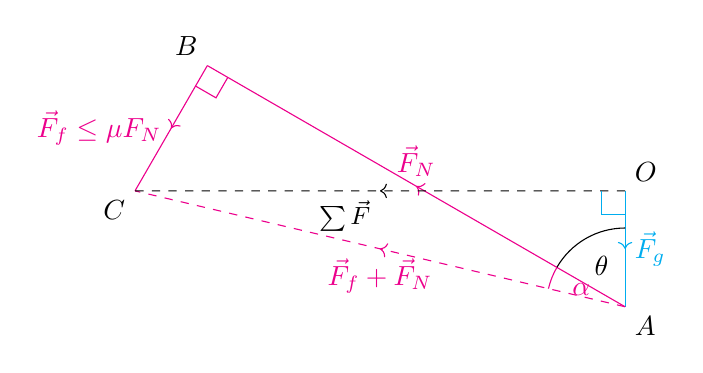
\begin{tikzpicture}[
            mid arrow/.style={
                postaction={decorate, decoration={
                    markings,
                    mark=at position 0.5 with {\arrow{>}}
                }}
            },
            resultant/.style={dashed, ->-}
        ]

            \pgfmathsetmacro{\radius}{2}
            \pgfmathsetmacro{\g}{9.81}
            \pgfmathsetmacro{\mass}{0.15}
            \pgfmathsetmacro{\incline}{60}
            \pgfmathsetmacro{\fric}{0.3}
            \pgfmathsetmacro{\speed}{sqrt(\radius * \g * ( (tan(\incline)+\fric)/(1-\fric*tan(\incline)) ))}

            \pgfmathsetmacro{\Fg}{\mass * \g}
            \pgfmathsetmacro{\FN}{\mass * ((\speed^2 * sin(\incline) / \radius) + (\g * cos(\incline)))}
            \pgfmathsetmacro{\Ff}{\mass * ((\speed^2 * cos(\incline) / \radius) - (\g * sin(\incline)))}

            \coordinate (O) at (0,0);
            \draw[mid arrow, cyan] (O) -- ++(0, -\Fg) coordinate (A) node[midway, right] {$\vec{F}_g$};
            \draw[mid arrow, magenta] (A) -- ++({90+\incline}:\FN) coordinate (B) node[midway, above] {$\vec{F}_N$};
            \draw[mid arrow, magenta] (B) -- ++({180+\incline}:\Ff) coordinate (C) node[midway, left] {$\vec{F}_f\le\mu F_N$};
            \draw[mid arrow, dashed, magenta] (A) -- (C) node[midway, below] {$\vec{F}_f+\vec{F}_N$};
            \draw[mid arrow, dashed] (O) -- (C) node[midway, below left, font=\small] {$\sum\vec{F}$};

            \pic [draw, "$\theta$", angle radius=1.0cm] {angle = O--A--B};
            \pic [draw, "$\alpha$", angle radius=1.0cm, magenta] {angle = B--A--C};
            \pic [draw, angle radius=0.3cm, cyan] {right angle = C--O--A};
            \pic [draw, angle radius=0.3cm, magenta] {right angle = A--B--C};

            \node[above right] at (O) {$O$};
            \node[below right] at (A) {$A$};
            \node[above left] at (B) {$B$};
            \node[below left] at (C) {$C$};

        \end{tikzpicture}
        \caption*{Case 1}
    \end{minipage}
    \begin{minipage}{0.4\textwidth}
        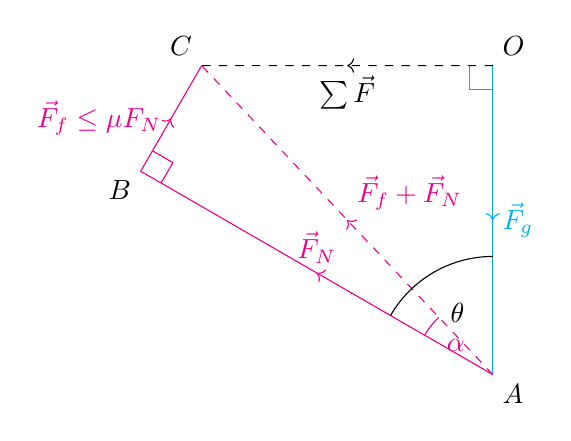
\begin{tikzpicture}[
            mid arrow/.style={
                postaction={decorate, decoration={
                    markings,
                    mark=at position 0.5 with {\arrow{>}}
                }}
            },
            resultant/.style={dashed, ->-}
        ]

            \pgfmathsetmacro{\radius}{2}
            \pgfmathsetmacro{\g}{9.81}
            \pgfmathsetmacro{\mass}{0.4}
            \pgfmathsetmacro{\incline}{60}
            \pgfmathsetmacro{\fric}{0.3}
            \pgfmathsetmacro{\speed}{sqrt(\radius * \g * ( (tan(\incline)-\fric)/(1+\fric*tan(\incline)) ))}

            \pgfmathsetmacro{\Fg}{\mass * \g}
            \pgfmathsetmacro{\FN}{\mass * ((\speed^2 * sin(\incline) / \radius) + (\g * cos(\incline)))}
            \pgfmathsetmacro{\Ff}{\mass * ((\speed^2 * cos(\incline) / \radius) - (\g * sin(\incline)))}

            \coordinate (O) at (0,0);
            \draw[mid arrow, cyan] (O) -- ++(0, -\Fg) coordinate (A) node[midway, right] {$\vec{F}_g$};
            \draw[mid arrow, magenta] (A) -- ++({90+\incline}:\FN) coordinate (B) node[midway, above] {$\vec{F}_N$};
            \draw[mid arrow, magenta] (B) -- ++({180+\incline}:\Ff) coordinate (C) node[midway, left] {$\vec{F}_f\le\mu F_N$};
            \draw[mid arrow, dashed, magenta] (A) -- (C) node[midway, above right] {$\vec{F}_f+\vec{F}_N$};
            \draw[mid arrow, dashed] (O) -- (C) node[midway, below] {$\sum\vec{F}$};

            \pic [draw, "$\theta$", angle radius=1.5cm] {angle = O--A--B};
            \pic [draw, "$\alpha$", angle radius=1.0cm, magenta] {angle = C--A--B};
            \pic [draw, angle radius=0.3cm, cyan] {right angle = C--O--A};
            \pic [draw, angle radius=0.3cm, magenta] {right angle = A--B--C};


            \node[above right] at (O) {$O$};
            \node[below right] at (A) {$A$};
            \node[below left] at (B) {$B$};
            \node[above left] at (C) {$C$};
        \end{tikzpicture}
        \caption*{Case 2}
    \end{minipage}
\end{figure}

As before, we combine the two cases in our calculations using ($\pm$). From the diagrams, we have:
\begin{align*}
    \tan(\theta\pm\alpha) &= \frac{|\sum\vec{F}|}{|F_g|} \qquad\qquad\because \triangle OAC \\ 
    \left|\sum \vec{F}\right| &= |F_g| \tan(\theta\pm\alpha) \\
    m\frac{v^2}{r}&=mg\tan(\theta\pm\alpha) \\ 
    \therefore |v| &= \sqrt{rg\tan(\theta\pm\alpha)}
\end{align*}

We now find the range of values for $\alpha$, which doesn't depend on the case:

\begin{align*}
    \tan\alpha &= \frac{|F|_f}{|F_N|} \\
    &\le \frac{\mu|F_N|}{|F_N|} \\ 
    &\le \mu \\ 
    \therefore 0\le\alpha &\le \arctan\mu
\end{align*}

When $\alpha$ is at max, $\tan(\theta+\alpha)$ is at max and $\tan(\theta-\alpha)$ is at min. Thus, we conclude:

\begin{center}
\boxed{\sqrt{rg\tan(\theta-\arctan\mu)}\le|v|\le\sqrt{rg\tan(\theta+\arctan\mu)}}
\end{center}

\section{New Business -- Lightnight McQuation}


\end{document}